A figura \ref{atividiagram} apresenta a aplicação das regras em termos de diagrama de atividades. Essa figura deve ser entendida como uma proposta de orientação das regras registradas na subseção \ref{regras}. Há outras maneiras de organizar essas regras em diferentes diagramas de estado. Contudo, a proposta presente neste modelo aponta para uma estrutura que corresponde as expectativas das semânticas do vocabulário aqui proposto.

O primeiro termo desta figura corresponde a "carregar todos os agentes". Esse elemento é indiferente a estrutura das regras do modelo. A existência desta atividade no diagrama se dá por finalidades de implementação, uma vez que para a uma máquina poder processar todos as atividades, primeiramente se faz necessário que informações sobre os agentes sejam carregadas na memória. As atividades "selecione um dos agentes", "carregar os objetivos", "há objetivos que não foram alcançados" e "o agente escolhe por tentar alcançar o objetivo" fazem referência as regras \ref{rolenextgoal} e \ref{reldeonticrole}. Aquela analisa qual é a próxima regra que esta em condições de serem atingidas pelo agente e esta verifica a permissão do agente no que tange a possibilidade de poder adotar o objetivo. 

O ponto de decisão "todas as condições necessárias para esse objetivo estão presentes?" e a atividade "violação de condição" fazem referência a regra \ref{violationcondition}, que define uma violação de condição para o caso do agente tentar executar alguma atividade sem que todas as condições estejam presentes naquele instante.

O ponto de decisão "todas as entidades necessárias para esse objetivo estão presentes?" e e atividade "violação de relação" fazem referência a regra \ref{violationentity}, pois definem o ocorrido no que diz respeito a ausência de uma entidade ao verificar um dado objetivo em análise. 

\begin{figure}[H]
  \centering
  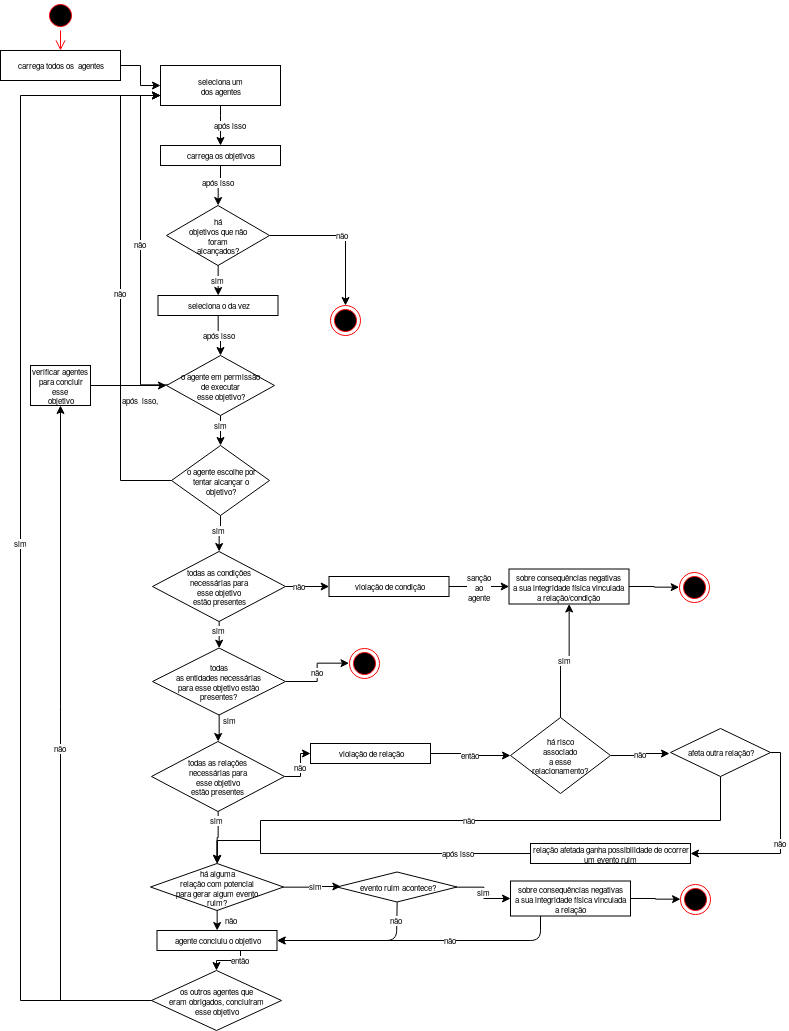
\includegraphics[width=1\linewidth]{figure/DiagramaDeAtividade.png} 
  \caption{Diagrama de atividades do modelo}
  \label{atividiagram}
\end{figure}

O ponto de decisão "todas as relações para esse objetivo estão presentes" e "violação de relação" representam a regra \ref{violationrelation}. Isso se deve ao fato de que essas atividades avaliam se uma das relações necessárias para cumprir com o objetivo não está presente resultando em uma violação de relacionamento. 

As atividades  "violação de condição" e "sobre consequências negativas a sua integridade física vinculada a relação/condição" condizem com a regra \ref{consviolationcondition} que define as consequências de uma violação de condição. A atividade "violação de relação" em conjunto com a segunda atividade das presentes na sentença anterior fazem referência a regra \ref{consviolationrelation}, pois apresenta as sanções relacionadas a uma violação de relacionamento. 

O ponto de decisão "há risco associado a esse relacionamento?", "afeta  outra relação" e "relação afetada ganha possibilidade de ocorrer um evento ruim" apontam para a regra \ref{violationrelationaffect} pois ambas situações representam como a ocorrência de uma violação de relacionamento afeta um outro relacionamento. A regra \ref{paybutiamnotguilty} corresponde aos seguintes aspectos do diagrama "há alguma relação com potencial para gerar algum evento ruim?", "evento ruim acontece?","sobre consequências negativas a sua integridade física vinculadas a relação" tendo em vista a equivalência semântica entre esses elementos sendo que ambas representações se preocupam com a análise de relações que possuem possibilidades de algum evento ruim surgir sobre o agente do objetivo. 

A regra \ref{consvioent} é representada por "violação de entidade" e o elemento que indica o fim do programa tendo em vista que ambas condições correspondem que na ocorrência deste evento, então a atividade deve ser encerrada.

Os eventos "agente concluiu o objetivo", "os outros agentes que eram obrigados, concluíram esse objetivo" e "verificar agentes para concluir esse objetivo" apontam para as regras \ref{rolenextgoal}, \ref{rolelastgoal}. Esse conjunto de atividades e pontos de decisões apresentam os critérios para definir quando um objetivo foi totalmente alcançado ou não assim como essas referidas regras.  A regra \ref{wenStop} é explicitada no diagrama toda vez que a atividade "sobre consequências negativas a sua integridade física vinculada a relação/condição" aponta para o fim do programa, tendo em vista que ambras representações representam o encerramento das atividades tendo em vista o surgimento de feridos. 

O diagrama \ref{atividiagram} demonstra \ref{violationcondition} é a primeira regra de violação a ser executada. O motivo disto reside no fato de que essa regra verifica se o agente respeitou todas as condições do ambiente. Se o agente não fizer isso, ele está sujeito a penalidades físicas encerrando o programa. Ou seja, não abre margens para verificação de outras violações, porque em um caso real, alguém que executa uma atividade sem que todas as condições estejam presentes, então esse alguém está fadado a encerrar qualquer ação em curso. Mesmo que esse alguém estivesse na condição de cometer outras violações, nunca seria possível fazer - pois esta primeira violação cometida por ele foi o suficiente para interromper os procedimentos como um todo. Esse mesmo principio fundamenta o sequenciamento das demais regras, sendo que logo em seguida é a \ref{violationentity} pois se alguma entidade não necessária (ferramenta) não estiver presente no cenário,então não existe possibilidade da continuidade dos procedimentos inviabilizando a realização das relações não fazendo sentido algum verificar \ref{violationrelation}. Contudo, os engenheiros definem essa estrutura apenas como uma proposta que deve ser modificada em função dos interesses da aplicação. Por exemplo, supondo que uma equipe tenha o interesse de usar este modelo para desenvolver jogos sérios com a intenção de analisar todas as violações que podem ser cometidas por um jogador sobre dado cenário, então para esse caso não há sentido usar esse fluxo de atividades. Em uma condição assim, os engenheiros do jogo devem - usando as mesmas regras - mudar o fluxo do diagrama de atividade para verificar todas as regras de violação antes de analisar se o programa deve ou não ser interrompido.